\section{Marco Teórico}

\subsection{Polarización de MosFets}

La curva de transferencia en los MosFets sigue la ecuación \ref{transferencia}, lo cual presenta una cierta dificultad a la hora de hacer el cálculo de polarización, ya que la corriente de salida no depende linealmente de la tensión de polarización. Es por esto que, como se discutirá en el diseño, se optó por resolver los circuitos por computadora.

\begin{equation}
  I_{DS} = K\cdot (V_{GS} - V_TH)^2
  \label{transferencia}
\end{equation}

Para hacer un modelado correcto del amplificador y poder resolverlo es necesario encontrar las ecuaciones que relacionen los parametros $V_{GS}$, $I_{DS}$ y $V_{DS}$ de cada transistor en el circuito (\ref{Amplificador Completo}).

\begin{figure}[H]
  \centering
  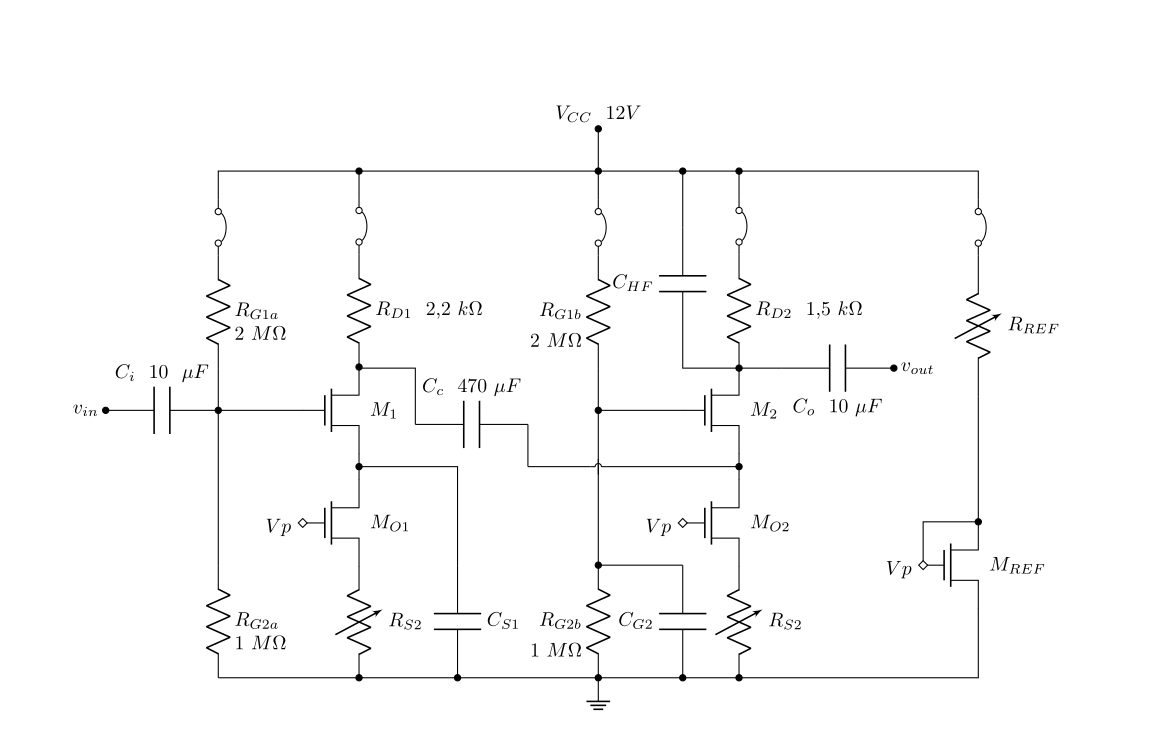
\includegraphics[width=\linewidth]{Imagenes/EsquematicoCatedra.png}
  \caption{Amplificador Completo}
  \label{Amplificador Completo}
\end{figure}

Encontrar esas relaciones implica conocer la relación entrada-salida de cada transistor ($V_{GS}$-$I_{DS}$) y la característica de salida ($I_{DS}$-$V_{DS}$), haciendo el análisis de mallas para encontrar las ecuaciones y poder calcular el punto de operación y las rectas de carga de los transistores.

El amplificador consta de dos etapas identicas en configuracón Fuente Común polarizadas con fuente de corriente (los transistores $M_{o1}$ y $M_{o2}$), por lo tanto, las rectas de carga solo se trazan para $M_{1}$ y $M_{2}$, ya que son estos los transistores amplificadores.

\subsubsection{Espejos de corriente}

La polarización con fuentes de corriente se logra con los espejos de corriente, que en este caso es fabricado con $M_{ref}$ y $R_{ref}$. Este transistor opera en una condición particular de polarización ($V_D = V_G$) y es polarizado únicamente por la resistencia $R_{ref}$. La $V_P = V_{Dref} = V_{Gref}$ es la tensión de polarización de $M_{o1}$ y $M_{o2}$ y es esto lo que forma el espejo de corriente. 

La corriente de $M_{ref}$ está fijada por $R_{ref}$, pero se relaciona con las corrientes de polarización de $M_{o1}$ y $M_{o2}$ (y, por consecuencia, de $M_{1}$ y $M_{2}$) con las resistencias variables de estos transistores. Esto permite lograr dos cosas, utilizar una fuente de corriente para polarizar los transistores amplificadores, lo que brinda una mayor estabilidad del punto Q, y modificar la ganacia total del amplificador variando un solo parámetro, $R_{ref}$.

La transconductancia de los MosFets es directamente proporcional a la corriente de drenaje, por lo que variando $R_{ref}$ es posible ajustar el valor de $I_{DSref}$, lo cual no tiene efecto directo en la ganancia, pero esto también varía las fracciones reflejadas de esta corriente en $M_{o1}$ y $M_{o2}$, que también son las de los transistores $M_{1}$ y $M_{2}$, que si tienen efecto en la ganancia. 

\subsection{Respuesta en Frecuencia}

El análisis de la ganancia se hace utilizando el modelo en pequeña señal de los transistores y considerando que el amplificador está operando en la banda media o de paso, donde los capacitores de baja frecuencia se comportan como cortocitcuito y los de alta frecuencia como un circuito abierto.

El cálculo y análisis de los capacitores de baja frecuencia se hace con este mismo modelo, para encontrar las frecuencias de corte de los capacitores se deben hacer algunas consideraciones antes de poder calcularlos. Se considera que un capacitor no tiene efecto sobre el resto cuando la frecuencia de su polo está alejada del resto en al menos tres octavas, idealmente una década, en estas condiciones es posible disernir el estado (alta o baja impedancia) del resto de capacitores con respecto al analizado.

En ocasiones, los capaciores del circuito están en mallas aisladas, por lo que no interactúan entre si y no es necesario tener esto en cuenta, en otros casos si están en la misma malla, por lo que, o se hace un análisis cualitativo previo para estimar cúal de los capacitores tendrá asociada una resistencia equivalente menor (este será el polo dominante) para disernir las condiciones del resto, o se tienen en cuenta todos los casos posibles y se anañizan los resultados de las frecuencias de corte para definir cuál es la condición correcta.

En el caso de baja frecuencia, los ceros se calculan como el inverso del producto entre el valor de capacitancia y la impedancia directamente asociada en paralelo, si esta no existe, como es el caso en los capacitores de desacoplo, esa impedancia es infinita y la frecuencia de corte es cero. Los polos se calculan como el inverso del producto entre la capacidad y la resistencia equivalente desde el capacitor analizado (equivalente de Thevenin).

El modelo en pequeña señal no alcanza para analizar el comportamiento en alta frecuencia del amplificador, ya que cobra relevancia el efecto de las capacidades parásitas de los transistores, por lo que es necesario considerarlas. Estas capacidades traen cosigo el efecto Miller, la reducción del ancho de banda a causa de una capacidad equivalente mayor a la parásita, dando una frecuencia de corte menor.

Si bien el modelo es distinto, la frecuencia del polo se calcula de la misma forma que en baja frecuencia, la distinción es que no hay ceros que contribuyan en alta frecuencia. En la función de transferencia las contribuciones de los ceros y polos en baja se expresan como $s + \omega_{Z}$ y $s + \omega_{P}$ y las de alta frecuencia como $1 + \frac{s}{\omega_{P}}$. La función de trasferencia de este amplificador se puede escribir como:

\begin{equation}
  A_{V}(s) = \frac{A_V \cdot s^3}{(s + \omega_{Co}) \cdot (s + \omega_{Cc}) \cdot (s + \omega_{Cs1}) \cdot (1 + \frac{s}{\omega_{Chf}})}
\end{equation}

La ausencia de $C_i$ y del posible polo en alta frecuencia generado por $M_1$ es debido a que, para simplificar el análisis, solo se tuvieron en cuenta las contribuciones en alta frecuencia de la última etapa, ya que el objetivo de $C_{hf}$ es limitar el ancho de banda, por lo que las contribuciones del capacitor parásito en alta de $M_1$ serían despreciables. Por otro lado, la resistencia equivalente de $C_i$ haría que su polo fuera despreciable, por lo que tampoco se tuvieron en cuenta sus contribuciones.



















